\chapter{Agent Development}
\label{cha:agent_development}

In this chapter we present the iterative development of the agent. We describe the
successive phases of its evolution, from the initial prototype to the final
implementation. During this process, several challenges and unexpected issues
emerged. For each phase, we detail the encountered problems and the approaches
adopted to overcome them, explaining the reasoning behind the design choices.
The majority of the choices taken in the crafting of the various prompt will be
discussed in Chapter \ref{cha:data_collection}, while reporting here all the discarded
ones.

\section{Development information}
\label{sec:development_information}

The go-to programming language for AI development is Python. However, we chose
to use JavaScript for this project for several reasons. First, both the server
and the example agents were already implemented in JavaScript; so a JavaScript interface
to communicate with the server was already available. This allowed us to focus
only on the agent's logic, without having to worry about the server's implementation.
Second, thanks to the availability of the project of the Autonomous Software Agents
course, our initial plan was to use an existing JavaScript-based benchmark from
the course. Although we ultimately decided against using this benchmark, as
explained later, JavaScript remained our language of choice.

Additionally, since there is no more a dedicated JavaScript library for the
Azure OpenAI API, instead of manually recreating the necessary API calls we opted
for a more efficient approach by setting up a lightweight Python server to act as
a middleman. This solution, discussed in Section \ref{par:azureapi}, allowed us
to integrate Azure's services seamlessly while maintaining JavaScript for the
core development.

\section{First Approach}
\label{sec:first_approach}

In this initial phase of the development and testing process, a trial-and-error
methodology was adopted to iteratively refine the system's behavior and try to
optimize performance. Unfortunately, this led to moving away from the definition
of the problem and, in combination with the poor performance of the agent, it
was decided to start over with a new approach. Nonetheless, this first attempt
was crucial in understanding the challenges and limitations of the problem, so it
is important to describe it.

\vspace{1mm}
\begin{codewindow}
  [Text] \lstset{style=pythonstyle, caption={Scheme of a prompt used in the first approach, full in Appendix \ref{lst:apx:first_agent_prompt}},
  label={lst:first_agent_prompt}} \begin{lstlisting}
[ROLE]

[MAP]

[LEGEND]

[ACTIONS]

[PARCELS ALREADY PICKED]

[RULES]

[QUESTION]
\end{lstlisting}
\end{codewindow}
\vspace{1mm}

The approach began by parsing crucial information from the server, which served as
the foundation for understanding how the LLM would interact with it. The main
point of discuss in the parsing topic was the map, that was represented as a multi-line
string like the one in Listing \ref{lst:parced_map}. The first prompt sent to
the LLM was crafted by concatenating the map with all the other information
needed to describe the state of the environment, as shown in Listing \ref{lst:first_agent_prompt}.

\vspace{1mm}
\begin{codewindow}
  [Text] \lstset{style=pythonstyle, caption={Parsed Map Result with partial legend},
  label={lst:parced_map}} \begin{lstlisting}
    1 1 1 1 1
    1 1 P 1 1
    1 1 1 1 1
    2 A 1 1 1
    1 1 1 1 1

    LEGEND:
    1: Walkable cell
    2: Delivery point
    A: Agent
    P: Parcel
\end{lstlisting}
\end{codewindow}
\vspace{1mm}

This implementation started as a full raw approach, letting the LLM also decide the
goal to pursue. As various challenges and inefficiencies were identified during
extensive testing, we progressively implemented a total of seven ``helping"
parameters.

\subsection{Helping Parameters}
These parameters were introduced with the objective of addressing specific
issues observed during experimentation, and each of them played a significant role
in shaping the overall functionality of the agent:
\begin{itemize}
  \item \texttt{ANTI\_LOOP}: This parameter was introduced to eliminate a common
    inefficiency in agent movement, wherein the agent would repeatedly traverse
    the same path in a circular loop, failing to make meaningful progress toward
    its goal. By setting this parameter to \texttt{true}, if the last four
    action were \texttt{["U", "R", "D", "L"]} (either clockwise or
    counterclockwise) the agent was forced to take an action that prevented the loop
    for happening. This optimization helped the agent make more intelligent
    movement decisions, thereby removing the possibility of being stuck in repetitive
    cycles;

  \item \texttt{HELP\_THE\_BOT}: The primary purpose of this parameter was to assist
    the agent in handling parcels more effectively. When activated by setting it
    to \texttt{true}, the agent was programmed to automatically take a parcel if
    the parcel was located directly below its current position. Additionally, if
    the agent was positioned at a delivery point, this parameter ensured that the
    agent would immediately proceed with shipping the parcel without requiring additional
    decision-making steps. This was implemented to reduce the number of calls to
    the LLM, since, even in this version of the agent, it was able to always pick
    up a parcel and deliver it (if in the correct tile);

  \item \texttt{SELECT\_ONLY\_ACTION}: This parameter was designed to simplify the
    agent's decision-making process in cases where the list of available actions
    contained only a single option. When set to \texttt{true}, the agent would
    automatically select and execute the sole available action without
    hesitation or delay. This was made by a big filtering phase that returned the
    legal actions:
    \begin{itemize}
      \item remove the opposite of the last action;

      \item remove all the action that was not possible (like going left while
        in the first column or going up while in the first row);

      \item remove the delivery action if the agent wasn't carrying a parcel and
        in a delivery point;

      \item remove the pick action if the agent was in a cell with no parcel.
    \end{itemize}
    This, in combination with the \texttt{HELP\_THE\_BOT} parameter, reduced the
    number of unnecessary calls to the LLM, thereby enhancing the agent's
    efficiency, but also giving the agent too little decision power;

  \item \texttt{USE\_HISTORY}: This parameter is the only one that was kept for all
    the future iterations (more on this in Section \ref{sec:stateful}). The role
    of this parameter was to decide whether each call to the LLM should contain
    only the current state of the environment of the entire message history. If set
    to \texttt{true}, the LLM would have access to the full conversation history,
    allowing it to make more informed decisions based on past interactions and
    events. This feature was particularly useful and powerful, but also with a
    big downside related to the LLM context length, that will be discussed in Chapter
    \ref{cha:conclusions};

  \item \texttt{REDUCED\_MAP}: This parameter was introduced to optimize the space
    the map occupied in the prompt by limiting the environment described as a slice
    of the full map and then scaling all the coordinates (of the agent and the
    parcels) treating the reduced map as the total map. The reduction in size
    was determined based on the maximum value between \texttt{PARCELS\_OBSERVATION\_DISTANCE}
    and \texttt{AGENTS\_OBSERVATION\_DISTANCE} (from Server Configuration File,
    see Section \ref{sub:server_configuration_event_handling}), ensuring that
    the agent only received the most relevant spatial data necessary for making
    informed decisions. Essentially, this optimization allowed the attention of
    the LLM to not be too sparse, but bringing some extra problems, for example
    by removing any delivery zone from the map since it was too far away while
    the current goal was to deliver a parcel;

  \item \texttt{HELP\_FIND\_DELIVERY}: This parameter was specifically designed to
    assist the agent in locating delivery points more effectively. By setting it
    to \texttt{true}, the system ensured that the closest delivery point (using Manhattan
    Distance) was always included in the agent's prompt (not as coordinates but as
    directions, eg. "right and up"), even if that particular delivery point was not
    within the agent's immediate field of view. In fact, this parameter was implemented
    to remedy the problem described in the \texttt{REDUCED\_MAP} point. This feature
    provided the agent with valuable directional guidance, allowing it to make
    better routing decisions and reducing the risk of wandering aimlessly in
    search of a delivery location (or worse, by looping again and again), but
    also reduced our ability to track the LLM ability in finding the delivery
    point by itself (more on this in Section \ref{sec:prompts});

  \item \texttt{HELP\_SIMULATE\_NEXT\_ACTIONS}: The goal of this parameter was to
    enhance the agent's decision-making process by simulating and displaying the
    expected outcomes of each possible action. When activated by setting it to
    \texttt{true}, the prompt provided to the LLM included a detailed breakdown
    of how each available action would alter the surrounding environment, by computing
    for each action the resulting map and attaching all of them to the final prompt.
    In theory, this additional information could help the agent anticipate and select
    the most favorable course of action. However, experimental results indicated
    that enabling this feature led to suboptimal performance, resulting in poor
    decision-making and inefficiencies, probably due to the size of the prompt that
    was too big for the LLM to handle.
\end{itemize}

This design resulted in an implementation that was bringing the project in the wrong
direction, because the whole ``no framework on top" idea was breaking down even if
this didn't have anything to do with planning in a strict sense. Without those
helps, the agent was not able to perform well in any environment, and the
decision was made to start over with a new approach.

Overall, while this initial approach did not yield the desired performance, it
was an essential step for the next iterations of the agent's development.

The code for this first implementation can be found in the \texttt{archive/raw\_llm\_agent.js}
file inside the project repository \cite{projectrepo}.

\subsection{Takeaways}
Through this initial approach, we gained valuable insights into the challenges
of designing an effective agent. The key lessons learned from this phase can be summarized
as follows.

\paragraph{Why this approach has been discarded?}
Several key issues made this method not suitable for the project's objectives:
\begin{itemize}
  \item Unclear prompt style: the way information was structured in the prompt
    was not optimal. This became particularly evident in the uncertainty computation,
    where the agent frequently exhibited high uncertainty in its actions;

  \item Over-reliance on helping parameter: providing excessive hints and
    structured input to the agent hindered its ability to explore the
    environment effectively. While guidance could be helpful, too much
    assistance made the results too distant from what the LLM could achieve by
    itself.
\end{itemize}

\paragraph{Key Takeaways from this phase}
\begin{itemize}
  \item Performance: when extensive guidance was provided, the results were still
    acceptable but inferior to those obtained using PDDL-based solutions.
    Initially, we considered implementing a PDDL version of the agent to serve as
    a benchmark. However, as discussed in Section \ref{sub:pddl_based_solutions},
    this comparison would have been unfair due to fundamental differences in
    approach and assumptions;

  \item Unintended biases in LLM behavior: Although not directly related to the
    core functionality of the agent, an interesting observation emerged regarding
    how the LLM interpreted the presence of other agents. The server allowed the
    spawning of ``enemy" agents capable of blocking paths. While this feature
    was not used in the main experiments, we discovered that simply including information
    about these agents in the prompt led the LLM to assume that agents near parcels
    were actively trying to steal them. In reality, these agents were merely obstacles
    with no intent to compete for parcels. This behavior highlights inherent
    biases in the LLM's training data, where similar context might have been associated
    with adversarial interactions.
\end{itemize}

\section{Second Approach}
\label{sec:second_approach}

In our exploration of different strategies for designing an LLM-driven agent,
this second approach was the weakest one. The fundamental idea was to adopt a "full
raw" approach, where the model received all available unprocessed data from the
server without any pre-processing or filtering. The hypothesis was that by exposing
the LLM to as much raw information as possible, it might be able to infer
meaningful patterns and determine the best course of action on its own, giving us
the ability to evaluate the LLM's planning capabilities without any external structure.
\vspace{1mm}
\begin{codewindow}
  [Text] \lstset{style=pythonstyle, caption={Scheme of a prompt used in the second approach, full in Appendix \ref{lst:apx:second_agent_prompt}},
  label={lst:second_agent_prompt}} \begin{lstlisting}
[ROLE]

Raw `onMap' response: [JSON]

Raw `onYou' response: [JSON]

Raw `onParcelsSensing' response: [JSON]

[ACTIONS]

[QUESTION]
\end{lstlisting}
\end{codewindow}
\vspace{1mm}

To achieve this, the agent's prompt was constructed as a simple collection of "name
of the call - JSON result" pairs. Unlike other approaches that structured data into
a more human-readable or semantically meaningful format, this method provided
the LLM with a direct dump of server responses. The only additional elements in the
prompt were the list of available actions and a loosely defined query requesting
the next step (necessary to compute the uncertainty).

At first glance, this approach seemed promising in that it completely avoided
manual interpretation of server responses, reducing the need for custom logic or
intermediate representations. If successful, it could have allowed for a highly adaptable
agent that functioned independently of predefined schemas or rigid data structures.

However, in practice, this approach performed poorly. While it occasionally
worked in very small maps, it became unreliable and inefficient as soon as the environment
grew even slightly more complex. The agent frequently took suboptimal paths, exhibited
excessive backtracking, and often failed to reach its goal efficiently.

Additionally, for the agent to work correctly in such small maps, the parameter
\texttt{USE\_HISTORY} from the first implementation was set to \texttt{true}, allowing
the LLM to leverage the `action-result' history.

The lack of structured guidance made it difficult for the model to consistently produce
useful responses, ultimately leading us to discard this approach in favor of
more refined strategies.

\subsection{Takeaways}

Even if this approach was the weakest one and has been discarded very soon, it
provided us with valuable insights into the limitations of the LLM in processing
raw data. The key lessons learned from this phase can be summarized as follows.

\paragraph{Why this approach has been discarded?}
\begin{itemize}
  \item Arbitrary Naming of API Calls: The names of server calls were not
    standardized and could change depending on the server's development. For instance,
    a call named "onMap" might return a list of map tiles, but there was no inherent
    guarantee of this behavior. Moreover, without explicit context, even
    we—humans—found it difficult to interpret certain responses;

  \item Lack of Context and Poorly Structured Input: The raw JSON data lacked
    structured context, making it challenging for the LLM to infer the correct course
    of action. Additionally, the query format itself was suboptimal. For example,
    if the prompt simply asked, "Go there, give me the next step to go there,"
    the model might struggle to determine that the immediate goal was not just
    reaching (x, y) but selecting the best intermediate step that moved the agent
    closer to that final destination.
\end{itemize}

\paragraph{Key Takeaways from this phase}
\begin{itemize}
  \item LLM Inference Capabilities: Surprisingly, the LLM was still able to extract
    some meaningful information from the unstructured data. While the results
    were inconsistent, there were instances where the model successfully inferred
    useful actions despite the messy prompt;

  \item Significant Impact of Prompt Engineering: Small modifications to the
    prompt led to drastic changes in the agent's behavior. This highlighted the critical
    role of prompt engineering in optimizing LLM performance, a topic we will
    explore in detail in Section \ref{sec:prompt_creation_choices}.
\end{itemize}

\section{Final Agent}
\label{sec:final_agent}

This represents the final iteration of our approach, incorporating substantial improvements
in both prompt generation and the overall structure of the agent's implementation.

Initially, prompts were dynamically constructed at runtime using a series of if/else
conditions, which made them difficult to manage, debug, and scale. That approach
lacked flexibility, as any modification required changes to the core logic of the
agent, increasing complexity and reducing maintainability.

\subsection{Prompt Management System}
In the revised approach, we transitioned to a structured prompt management system
where predefined templates are stored in a dedicated folder (\texttt{prompts} folder
in the GitHub repository \cite{projectrepo}). These templates use variable placeholders
that are replaced dynamically via regex-based substitutions. This change
provided multiple advantages: it improved readability, ensured consistency
across different prompts, and made modifications significantly easier. Instead
of altering the logic of the agent itself, changes could now be made directly at
the prompt level, allowing for rapid experimentation and iteration. Additionally,
this structured approach facilitated more systematic testing, as different versions
of the prompts could be evaluated with minimal effort. Overall, this refinement not
only enhanced the reliability of the agent but also contributed to a more efficient
development workflow.

\subsection{Agent Refactoring}
Beyond improving prompt handling, a major structural refactoring was undertaken
to optimize the agent's implementation. The original codebase was relatively monolithic,
with large, complex functions handling multiple aspects of decision-making. This
made debugging and extending functionality cumbersome. In the final version, the
implementation was restructured into a more modular design, with a greater number
of smaller, well-defined functions handling specific tasks. This decomposition significantly
reduced code redundancy, improved readability, and made the agent easier to modify.
One of the key benefits of this modular approach was its impact on the data
acquisition process. Since the agent's core logic was now more flexible,
adapting it for different data collection tasks required minimal effort. Simple function
modifications or prompt adjustments were often sufficient to tailor the agent's behavior
to new requirements. This ability to rapidly reconfigure the agent streamlined
experimentation and allowed us to gather diverse datasets efficiently, ultimately
improving the quality and scope of our evaluations.

\subsection{RAG Experiments}
We also explored the potential of Retrieval-Augmented Generation (RAG) as a way to
enhance the agent's decision-making process. The initial idea was to categorize
the parcels \emph{a posteriori} based on predefined classes and provide the LLM with
priority information for each category (example in Listing
\ref{lst:parcel_categorization}). This would have allowed the model to make more
informed decisions by leveraging structured context about the importance of
different types of parcels. However, while this approach showed promise, it was ultimately
considered too far from the core objectives of this thesis and was therefore not
pursued further.

\vspace{1mm}
\begin{codewindow}
  [JavaScript Code] \lstset{style=jsstyle, language=JavaScript, caption={Discarded implementation of an example of \emph{a posteriori} parcel categorization},
  label={lst:parcel_categorization}} \begin{lstlisting}
if (PARCEL_CATEGORIZATION) {
  for (let parcel of rawOnParcelsSensing) {
    const parcelIdNumber = parseInt(parcel.id.substring(1));
    parcel.food = parcelIdNumber % 2 === 0 ? "banana" : "pineapple";
  }
}
\end{lstlisting}
\end{codewindow}
\vspace{1mm}

Another experimental RAG-based approach involved providing the agent with direct
information about past actions, such as: ``The last time you were in position\texttt{(x,
y)}, you attempted to move up, but the path was blocked". While this could be a
useful strategy for a ``blind" agent (one without direct state awareness) its application
in our case would have led to a problematic behavior. The agent would work by
just performing random actions, gathering information about the blocked/suboptimal
paths and then relying entirely on the RAG-generated feedback to navigate. This
effectively bypassed the agent's core decision-making process, turning it into a
reactive system rather than a proactive one. Given our focus on autonomous
decision-making, this approach was deemed unsuitable.

Nonetheless, these experiments highlighted the potential of RAG for different
types of autonomous agents and may be worth exploring in future research.

\subsection{Stateless and Stateful Agents}

The final agent played a crucial role in generating the heatmaps discussed in Section
\ref{sec:uncertainty_visualization}, primarily leveraging GPT-4o-mini. Task categorization
into \texttt{pickup} and \texttt{delivery} was handled by computing the number of
parcels currently in possession of the agent, rather than inferred dynamically
from the environment state. While an automated approach could have been explored,
manually assigning these tasks ensured clarity and allowed for more controlled
testing conditions.

Both stateless and stateful configurations of the agent were developed and
tested. The stateless version made decisions based solely on the current state,
while the stateful version incorporated historical context to refine its choices
over time thanks to the \texttt{action-result} feedback in the conversation history.

\subsection{Uncertainty Handling}
\label{sub:uncertainty_handling} To handle uncertainty in decision-making, we
experimented with three different approaches:
\begin{itemize}
  \item \textbf{Raw probability selection}: The agent directly selected the action
    with the highest probability, without any additional modifications. This approach
    was straightforward, but led to suboptimal (or totally wrong) paths when the
    highest-probability action was incorrect;

  \item \textbf{Weighted selection}: Instead of always choosing the most probable
    action, the agent sampled actions based on their probabilities. This method was
    particularly effective in the stateful configuration: if an incorrect action
    initially had the highest probability, randomness allowed the agent to eventually
    correct itself over multiple iterations on the same spot;

  \item \textbf{Stopping mechanism}: This approach follows literally the process
    explained in the paper `Robots That Ask For Help: Uncertainty Alignment for Large
    Language Model Planners' (explained in Section \ref{ssub:tokens_log_probability}):
    by filtering the actions after the computation of the scaled log-probability
    of each action, if the resulting set of possible actions was not a singleton
    the agent would stop waiting for the user input. This method was implemented
    for completeness in the development, but not tested automatically since it
    would have required human intervention.
\end{itemize}
Among these methods, weighted selection proved to be the most effective for data
acquisition and testing, as it leveraged randomness to improve path accuracy.
This experiment demonstrated that even when an LLM-based agent lacks perfect
reasoning abilities, incorporating controlled stochasticity can help guide it toward
better long-term performance.

\subsection{Takeaways}

We can summarize the biggest improvements in the final agent as ``prompt
management'' and ``agent refactoring''. The key lessons learned from this phase can
be summarized as follows.\\The change in the prompt management provided multiple
advantages:
\begin{itemize}
  \item Improved readability: The separation of logic from text made prompts
    easier to understand and modify;

  \item Consistency and maintainability: Storing prompts as templates reduced
    duplication and made debugging simpler;

  \item Faster experimentation: Changes could be made at the prompt level
    without modifying the agent's core logic;

  \item Better testing and evaluation: Different prompt versions could be
    systematically compared with minimal effort.
\end{itemize}
The refactoring of the agent structure also brought several advantages:
\begin{itemize}
  \item More modular design: Smaller, well-defined functions improved readability
    and maintainability;

  \item Reduced code redundancy: Reusable components simplified implementation
    and debugging;

  \item Greater flexibility: The agent could be easily adapted for new tasks, making
    data acquisition faster and more efficient.
\end{itemize}

\section{Extra: Closest Cell to the Goal}
\label{sec:closest_cell_to_the_goal}

As part of the iterative process of refining our agent, we also tried to systematically
isolate and address specific challenges by progressively reducing the complexity
of the final problem. This incremental approach not only helped us pinpoint
potential weaknesses in the agent's decision-making process but also provided
deeper insights into the LLM's underlying behaviors and limitations.

To achieve this, we conducted a series of controlled experiments, including:
\begin{itemize}
  \item \textbf{Testing on smaller, simplified maps}: By reducing environmental complexity,
    we could more easily observe the agent's decision-making patterns and
    identify whether failures were due to reasoning errors or external factors;

  \item \textbf{Using custom, ``disposable" prompts}: We introduced minor variations
    in prompt structures to assess how sensitive the LLM was to different formulations
    of the problem. This helped us determine whether misinterpretations were
    caused by the model itself or by the way the information was presented;

  \item \textbf{Decomposing the final goal into smaller, manageable sub-goals}: Breaking
    down the problem into intermediate objectives allowed us to test whether the
    agent could handle incremental progress rather than needing to solve the entire
    task at once. This approach is further detailed in the following paragraphs.
\end{itemize}

One key issue we wanted to investigate was why the agent often failed to select
the optimal action leading toward the goal. Was the model inherently incapable of
making the correct choice, or was the issue rooted in the way the prompt was
structured? To better understand this, we designed an experiment that introduced
a two-step decision-making process (visible in Figure \ref{fig:extra}):
\begin{itemize}
  \item \textbf{Identifying the best neighboring tile}: Before making a move,
    the agent was first asked to determine the most optimal adjacent tile to
    step toward, effectively transforming the problem into a local optimization task;

  \item \textbf{Selecting the best action to reach that tile}: Once the target tile
    was identified, the agent was then tasked with choosing the appropriate
    action to move in that direction.
\end{itemize}

\vspace{7mm}
\begin{figure}[h!]
  \centering
  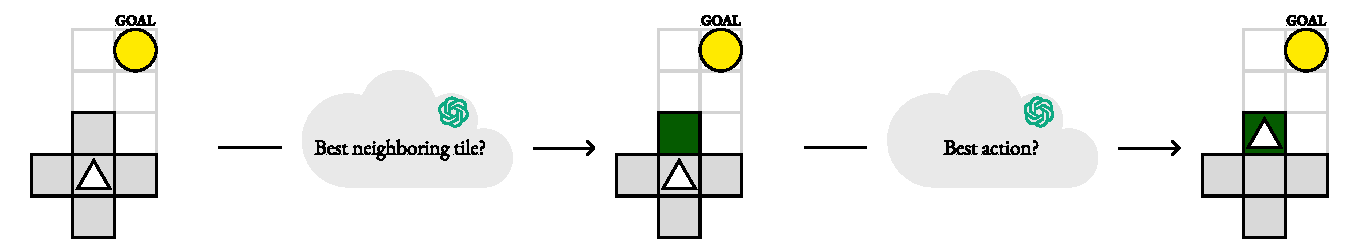
\includegraphics[width=\textwidth]{images/extra.pdf}
  \caption{Two-steps decision making example}
  \label{fig:extra}
\end{figure}
\vspace{7mm}

This method effectively reframed the problem from a complex, global pathfinding
challenge into a series of simpler, localized decisions. We hypothesized that
this decomposition would improve performance by reducing the cognitive load on
the LLM and allowing it to focus on smaller, well-defined tasks.

However, despite these modifications, the results did not align with our expectations.
The primary issue was that if the agent misidentified the best neighboring tile
by choosing a position that actually increased the distance to the goal, then even
a perfectly chosen direction would still lead to suboptimal behavior.

Another significant factor was the role of uncertainty computation in the LLM response.
When relying on the raw output of the LLM (`Raw probability selection' in Section
\ref{sub:uncertainty_handling}), results were often inconsistent or outright incorrect.
To address this, we experimented also with the uncertainty-weighted random action
selection approach (`Weighted selection' in Section
\ref{sub:uncertainty_handling}), where decisions were influenced by the model's
confidence levels. Unfortunately, this introduced additional challenges, as interpreting
the results became even more complex.

Ultimately, this experiment underscored the limitations of LLM-based decision-making
in logistics scenarios where local optimizations must align with global
objectives. The agent's inability to consistently select the correct neighboring
tile demonstrated how small errors at the decision-making level could compound,
leading to inefficient or even counterproductive actions.

However, as we will explore in Chapter \ref{cha:results_discussion}, newer LLM
models exhibit notable improvements in our task, suggesting that continued advancements
in the technology may help overcome these challenges and enhance overall performance
in complex logistics tasks.